\documentclass[crop=true, tikz=true, border={0.1cm 1cm 1cm 0.1cm}]{standalone}

\usepackage{times}
\usepackage{helvet}
\usepackage{courier}
\usepackage{url}  %Required
\usepackage{graphicx}  %Required

%%%%%%%%%%%%%%%%%%%%%
%%%% Packages
\usepackage{amsthm,amsmath,amssymb}
%\usepackage{tikz}
\usetikzlibrary{matrix}
\usepackage{pgf-umlsd}
\usepackage{pgfplots}
\usepackage{pgfplotstable}
\usepgfplotslibrary{fillbetween}
\usepackage{ragged2e}
\usetikzlibrary{arrows,automata,fit,calc,positioning,shapes,shapes.multipart} %
%\usepackage[inline]{enumitem}
\usepackage{enumerate,url,soul}
\usepackage{paralist}
%\usepackage[usenames]{color} % Only used in comment commands
\usepackage[ruled,vlined]{algorithm2e}
\usepackage{thmtools,thm-restate}
\usepackage{listings}
\usepackage{subcaption}
\usepackage{arydshln}

%definition environment
%\newtheorem{mydef}{Definition}[chapter]
%\newtheorem{myexp}{Example}[chapter]
%\newtheorem{mytheo}{Theorem}[chapter]

\newcolumntype{L}[1]{>{\raggedright\arraybackslash}p{#1}}
\newcolumntype{C}[1]{>{\centering\arraybackslash}p{#1}}
\newcolumntype{R}[1]{>{\raggedleft\arraybackslash}p{#1}}

\definecolor{mygreen}{HTML}{009933}

\newcommand{\abseq}{/\hspace{-0.18cm}\sim^\alpha}

\newcommand{\titledate}[2][2.5in]{%
  \noindent%
  \begin{tabular}{@{}p{#1}@{}}
    \\ \hline \\[-.75\normalbaselineskip]
    #2
  \end{tabular}
}

\renewcommand{\textfraction}{0.05}

\usepackage{geometry}
%\geometry{
%paperwidth=215mm,
%paperheight=27cm,
%margin=0.5cm
%}

\newlength{\mywidth}
\setlength{\mywidth}{16.5cm}

\begin{document}

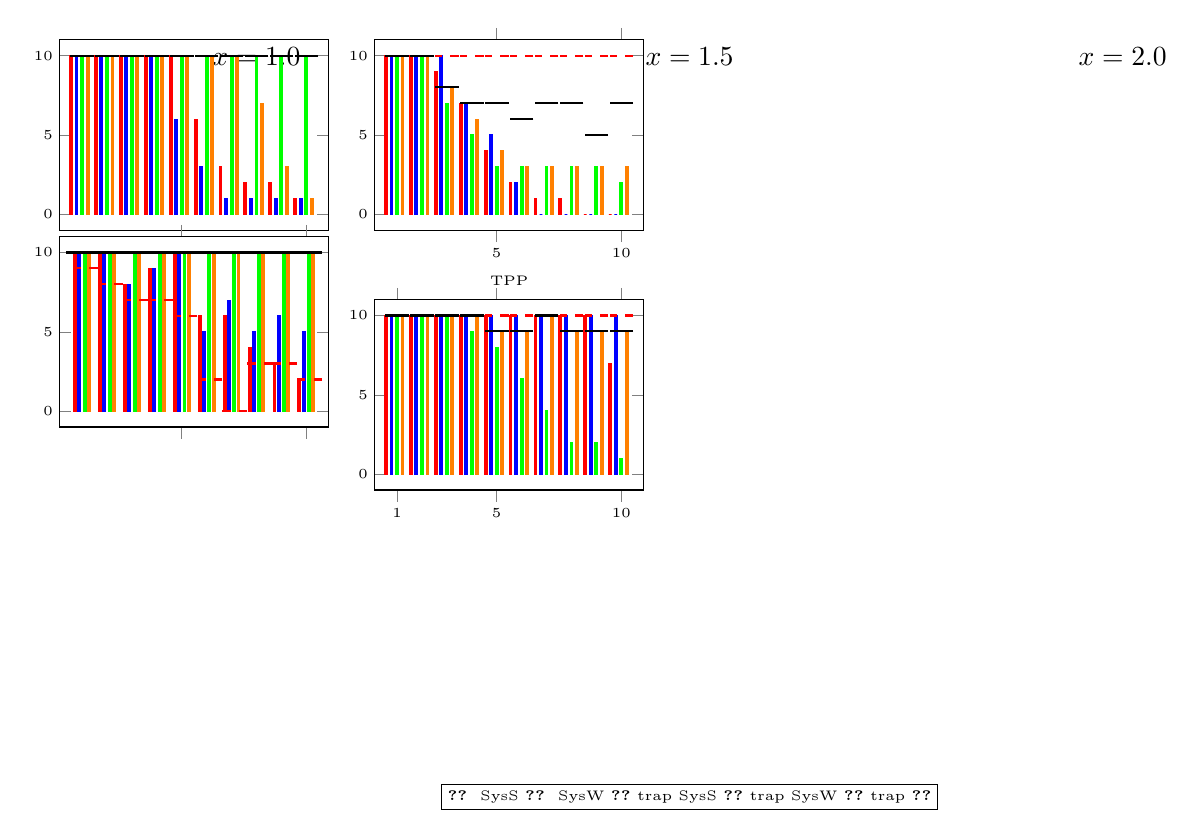
\begin{tikzpicture}
\node[] (c1) at (2.5,2.2) {$x=1.0$};
\node[] (c15) at (8,2.2) {$x=1.5$};
\node[] (c2) at (13.5,2.2) {$x=2.0$};


\tiny
    \begin{axis}[
    width =5cm,
    height=4cm,
    enlarge x limits = 0.1,
    enlarge y limits = 0.1,
    legend columns=1,
    ybar,
    bar width=1pt,
    ymin = 0,
    ymax = 10,
	compat=1.6,
	%title=c 100,
	%ylabel=goals 05,
	xticklabels={,,},
	xtick style={draw=none},
	at={(0,0)},
]
\addplot+[ybar, bar shift =-4.0pt, red,
]
plot coordinates {
(04, 10) %c_100
(05, 10) %c_100
(06, 6) %c_100
(01, 10) %c_100
(02, 10) %c_100
(08, 2) %c_100
(07, 3) %c_100
(03, 10) %c_100
(09, 2) %c_100
(10, 1) %c_100
};
\label{plot:props_bu_hff_94}
\addplot+[ybar, bar shift =-2.0pt, blue,
]
plot coordinates {
(04, 10) %c_100
(05, 6) %c_100
(06, 3) %c_100
(01, 10) %c_100
(02, 10) %c_100
(08, 1) %c_100
(07, 1) %c_100
(03, 10) %c_100
(09, 1) %c_100
(10, 1) %c_100
};
\label{plot:props_td_hff_94}
\addplot+[ybar, bar shift =0.0pt, green,
]
plot coordinates {
(04, 10) %c_100
(05, 10) %c_100
(06, 10) %c_100
(01, 10) %c_100
(02, 10) %c_100
(08, 10) %c_100
(10, 10) %c_100
(03, 10) %c_100
(09, 10) %c_100
(07, 10) %c_100
};
\label{plot:props_bu_trap_94}
\addplot+[ybar, bar shift =2.0pt, orange,
]
plot coordinates {
(04, 10) %c_100
(05, 10) %c_100
(06, 10) %c_100
(01, 10) %c_100
(02, 10) %c_100
(08, 7) %c_100
(07, 10) %c_100
(03, 10) %c_100
(09, 3) %c_100
(10, 1) %c_100
};
\label{plot:props_td_trap_94}

%lmcut
\addplot+[only marks, mark = -, mark options = {thick, red, dashed}, mark size = 0.15cm, black,
]
plot coordinates {
(01, 10)
(02, 10)
(03, 10)
(04, 10)
(05, 10)
(06, 10)
(07, 10)
(08, 10)
(09, 10)
(10, 10)
};

%trap first meta node top down
\addplot+[only marks, mark = -, mark options = {thick, black}, mark size = 0.15cm, black,
]
plot coordinates {
(01, 10)
(02, 10)
(03, 10)
(04, 10)
(05, 10)
(06, 10)
(07, 10)
(08, 10)
(09, 10)
(10, 10)
};

    \end{axis}
    \hfill
    
%\node[draw, align=center] (test) at (8,-18) {
%\ref{plot:props_bu_hff_94} props-bu-hff\\
%\ref{plot:props_td_hff_94} props-td-hff\\
%\ref{plot:props_bu_trap_94} props-bu-trap\\
%\ref{plot:props_td_trap_94} props-td-trap\\
%};

    \begin{axis}[
    width = 5cm,
    height=4cm,
    enlarge x limits = 0.1,
    enlarge y limits = 0.1,
    legend columns=1,
    ybar,
    bar width=1pt,
    ymin = 0,
    ymax = 10,
compat=1.6,
%title=c 150,
%ylabel=goals 6,
at={(4cm,0)},
]
\addplot+[ybar, bar shift =-4.0pt, red,
]
plot coordinates {
(08, 1) %c_150
(09, 0) %c_150
(03, 9) %c_150
(06, 2) %c_150
(07, 1) %c_150
(10, 0) %c_150
(04, 7) %c_150
(05, 4) %c_150
(01, 10) %c_150
(02, 10) %c_150
};
\label{plot:props_bu_hff_75}
\addplot+[ybar, bar shift =-2.0pt, blue,
]
plot coordinates {
(08, 0) %c_150
(09, 0) %c_150
(03, 10) %c_150
(06, 2) %c_150
(07, 0) %c_150
(10, 0) %c_150
(04, 7) %c_150
(05, 5) %c_150
(01, 10) %c_150
(02, 10) %c_150
};
\label{plot:props_td_hff_75}
\addplot+[ybar, bar shift =0.0pt, green,
]
plot coordinates {
(08, 3) %c_150
(09, 3) %c_150
(03, 7) %c_150
(06, 3) %c_150
(07, 3) %c_150
(10, 2) %c_150
(04, 5) %c_150
(05, 3) %c_150
(01, 10) %c_150
(02, 10) %c_150
};
\label{plot:props_bu_trap_75}
\addplot+[ybar, bar shift =2.0pt, orange,
]
plot coordinates {
(08, 3) %c_150
(09, 3) %c_150
(10, 3) %c_150
(06, 3) %c_150
(07, 3) %c_150
(03, 8) %c_150
(04, 6) %c_150
(05, 4) %c_150
(01, 10) %c_150
(02, 10) %c_150
};
\label{plot:props_td_trap_75}

%lmcut
\addplot+[only marks, mark = -, mark options = {thick, red, dashed}, mark size = 0.15cm, black,
]
plot coordinates {
(02, 10)
(01, 10)
(04, 10)
(03, 10)
(07, 10)
(08, 10)
(06, 10)
(10, 10)
(05, 10)
(09, 10)
};

%trap first meta node top down
\addplot+[only marks, mark = -, mark options = {thick, black}, mark size = 0.15cm, black,
]
plot coordinates {
(01, 10)
(02, 10)
(03, 8)
(04, 7)
(05, 7)
(06, 6)
(07, 7)
(08, 7)
(09, 5)
(10, 7)
};
    \end{axis}
    \hfill
    
%\node[draw, align=center] (test) at (8,-18) {
%\ref{plot:props_bu_hff_75} props-bu-hff\\
%\ref{plot:props_td_hff_75} props-td-hff\\
%\ref{plot:props_bu_trap_75} props-bu-trap\\
%\ref{plot:props_td_trap_75} props-td-trap\\
%%};


\begin{axis}[
width = 5cm,
height=4cm,
enlarge x limits = 0.1,
enlarge y limits = 0.1,
legend columns=1,
ybar,
bar width=1pt,
ymin = 0,
ymax = 10,
compat=1.6,
at={(0,-2.5cm)},
xticklabels={,,}
]
\addplot+[ybar, bar shift =-2.5pt, red,
]
plot coordinates {
(08, 4)
(09, 3)
(01, 10)
(03, 8)
(02, 10)
(04, 9)
(05, 10)
(06, 6)
(10, 2)
(07, 6)
};
\label{plot:properties_hff_bu_52}
\addplot+[ybar, bar shift =-1.0pt, blue,
]
plot coordinates {
(01, 10)
(08, 5)
(02, 10)
(04, 9)
(03, 8)
(05, 10)
(06, 5)
(10, 5)
(07, 7)
(09, 6)
};
\label{plot:properties_hff_td_52}
\addplot+[ybar, bar shift =1.0pt, green,
]
plot coordinates {
(09, 10)
(01, 10)
(02, 10)
(04, 10)
(03, 10)
(05, 10)
(06, 10)
(10, 10)
(07, 10)
(08, 10)
};
\label{plot:properties_trap_prefop_bu_52}
\addplot+[ybar, bar shift =2.5pt, orange,
]
plot coordinates {
(01, 10)
(08, 10)
(02, 10)
(03, 10)
(04, 10)
(05, 10)
(06, 10)
(10, 10)
(07, 10)
(09, 10)
};
\label{plot:properties_trap_prefop_td_52}

%start node sysW
\addplot+[only marks, mark = -, mark options = {thick}, mark size = 0.2cm, black,
]
plot coordinates {
(02, 10)
(01, 10)
(04, 10)
(03, 10)
(07, 10)
(08, 10)
(06, 10)
(10, 10)
(05, 10)
(09, 10)
};
%optimal
\addplot+[only marks, mark = -, mark options = {thick, red, dashed}, mark size = 0.2cm, black,
]
plot coordinates {
(03, 7)
(05, 6)
(07, 0)
(09, 3)
(01, 9)
(02, 8)
(04, 7)
(06, 2)
(08, 3)
(10, 2)
};

\end{axis}


    \begin{axis}[
    width = 5cm,
    height=4cm,
    enlarge x limits = 0.1,
    enlarge y limits = 0.1,
    legend columns=1,
    ybar,
    bar width=1pt,
    ymin = 0,
    ymax = 10,
	compat=1.6,
	at={(4cm,-3.3cm)},
	title=TPP,
	title style={yshift=-1.5ex},
	xtick= {1,5,10},
]
\addplot+[ybar, bar shift =-4.0pt, red,
]
plot coordinates {
(08, 10) %c_200
(05, 10) %c_200
(04, 10) %c_200
(10, 7) %c_200
(07, 10) %c_200
(06, 10) %c_200
(09, 10) %c_200
(03, 10) %c_200
(02, 10) %c_200
(01, 10) %c_200
};
\label{plot:props_bu_hff_44}
\addplot+[ybar, bar shift =-2.0pt, blue,
]
plot coordinates {
(08, 10) %c_200
(05, 10) %c_200
(04, 10) %c_200
(10, 10) %c_200
(07, 10) %c_200
(06, 10) %c_200
(09, 10) %c_200
(03, 10) %c_200
(02, 10) %c_200
(01, 10) %c_200
};
\label{plot:props_td_hff_44}
\addplot+[ybar, bar shift =0.0pt, green,
]
plot coordinates {
(08, 2) %c_200
(05, 8) %c_200
(04, 9) %c_200
(10, 1) %c_200
(07, 4) %c_200
(06, 6) %c_200
(09, 2) %c_200
(03, 10) %c_200
(02, 10) %c_200
(01, 10) %c_200
};
\label{plot:props_bu_trap_44}
\addplot+[ybar, bar shift =2.0pt, orange,
]
plot coordinates {
(08, 9) %c_200
(05, 9) %c_200
(04, 10) %c_200
(03, 10) %c_200
(07, 10) %c_200
(06, 9) %c_200
(09, 9) %c_200
(10, 9) %c_200
(02, 10) %c_200
(01, 10) %c_200
};
\label{plot:props_td_trap_44}

%lmcut
\addplot+[only marks, mark = -, mark options = {thick, red, dashed}, mark size = 0.15cm, black,
]
plot coordinates {
(02, 10)
(01, 10)
(04, 10)
(03, 10)
(07, 10)
(08, 10)
(06, 10)
(10, 10)
(05, 10)
(09, 10)
};

%trap first meta node top down
\addplot+[only marks, mark = -, mark options = {thick, black}, mark size = 0.15cm, black,
]
plot coordinates {
(01, 10)
(02, 10)
(03, 10)
(04, 10)
(05, 9)
(06, 9)
(07, 10)
(08, 9)
(09, 9)
(10, 9)
};
    \end{axis}
    \hfill
    
%\node[draw, align=center] (test) at (8,-18) {
%\ref{plot:props_bu_hff_44} props-bu-hff\\
%\ref{plot:props_td_hff_44} props-td-hff\\
%\ref{plot:props_bu_trap_44} props-bu-trap\\
%\ref{plot:props_td_trap_44} props-td-trap\\
%};




\node[draw] (test) at (8,-7.2) {
\ref{plot:properties_hff_bu_39} $\hff$ SysS
\ref{plot:properties_hff_td_39} $\hff$ SysW
\ref{plot:properties_trap_prefop_bu_39} trap SysS
\ref{plot:properties_trap_prefop_td_39} trap SysW
\ref{plot:baseline_sysW_node} trap
\ref{plot:baseline_lmcut} \hlmcut 
};
\end{tikzpicture}

\end{document}
